\mysubsection{Linda Schey}{Multimonitor Support}

Zu Beginn des Projektes wurde versuch eine möglichst große Projektionsfläche zu erhalten. In Ermangelung eines Beamer, der die gewünschte Größe projizieren konnte wurde auf drei Beamer zurückgegriffen, die dann nebeneinander ein jeder ein Drittel der Applikation darstellen sollte. Um dies zu realisieren musste aber das komplette Bild das projiziert werden sollte in drei einzelne Bilder geteilt. Da die Beamer nicht nebeneinander, sondern über einander aufgebaut werden sollten, damit das komplette Bild hoch und breit genug ist müssen die erhaltenen Bilder jeweils um 90° gedreht werden. Dafür wurde in Unity eine extra Kamera in die Szene eingefügt, die die Szene als RenderTexture aufnimmt. Diese RenderTexture wurde dann in drei einzelne Texturen getrennt. Jede Textur um 90° gedreht und dann nebeneinander als Gui-Elemente dargestellt. Soweit war diese Funktionalität auch schon implementiert, bis auf kleine Justierungen beim Zuschneiden der einzelnen Teil Texturen. \\
Ein anderer Ansatz war drei um 90° gedrehte Kameras in die Szene zu integreren die jeweils ein Drittel des Spielfeldes filmten. 
\begin{figure*}[h]
	\centering
		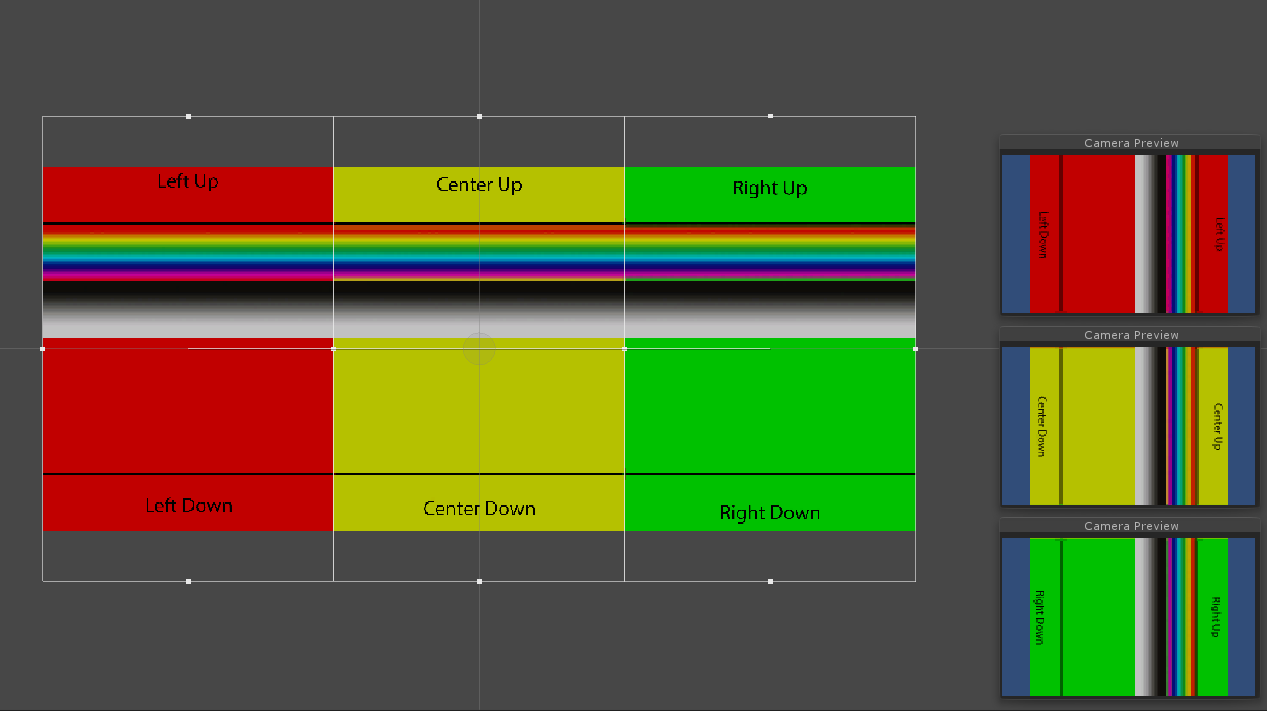
\includegraphics[width=0.8\textwidth]{images/RenderTextureBeispielSzene.PNG}
	\caption{Aufbau der Szene in Unity mit den drein RenderTextrure Ausschnitten am Beispiel eines Dummy Objektes}
	\label{fig:RenderTextureBeispielSzene}
\end{figure*}
Daraus erhielt man drei RenderTextures, die dann nebeneinander als Gui rendern werden konnten. Dafür wurde zunächst mit einem Beispiel Objekt gearbeitet, das ein Material zugewiesen bekam, welches es bei der Entwicklung vereinfachte zu erkenne, ob die Kameras richtig ausgerichtet waren und dann auch entsprechend richtig auf die Gui gerendert wurden. 
\begin{figure*}[h]
	\centering
		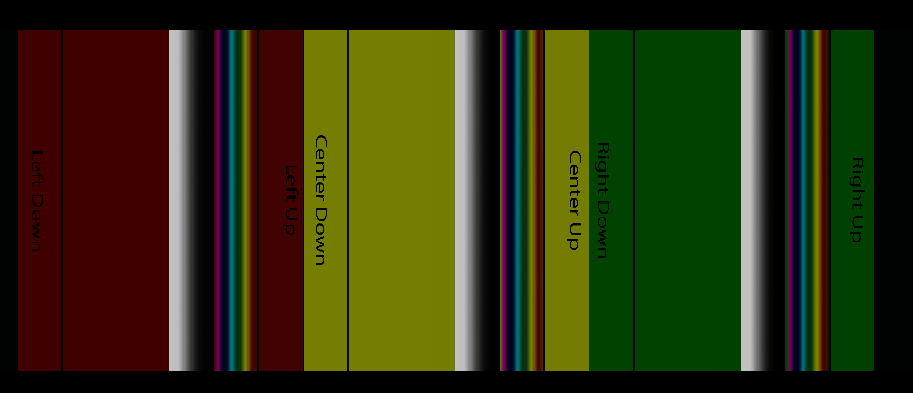
\includegraphics[width=0.8\textwidth]{images/RenderTexturesAlsGui.PNG}
	\caption{RenderTextures nebeneinander auf die Gui gerendert}
	\label{fig:RenderTexturesAlsGui}
\end{figure*}\\
Die drei Kameras, mussten jedoch von Hand auf die Szene eingestellt werden, so dass es auch hier wieder zu Ungenauigkeiten hätte kommen können. Andererseits wäre man hier flexibler beim Ausrichten der Szene auf die drei Beamer gewesen, in dem man zum Beispiel die Übergänge zwischen den drei Texturen jeweils so hätte Platzieren können, dass sie auf einem Spalt der Felder des Spielfeldes gelegen wären.\\ 
Beide Ansätze waren jedoch nicht zu 100 Prozent exakt,was das Aufteilten der Szene in drei Teil Texturen betraf. Außerdem standen keine drei identischen Beamer zur Verfügung, sodass es unter den einzelnen Beamern Unterschiede bei der Lichtintensität gab.
Da anstatt der Lösung mit den drei Beamern doch noch ein geeignetes Gerät gefunden wurde, das alleine die gewünschte Projektionsfläche erbrachte, wurde die Idee mit den drei Beamern, sowie die bisherige Implementierung dafür verworfen und ist im finalen Stand des Projektes nicht mehr enthalten.\\